% OLD VERSION IS COMMENTED OUT; NEW VERSION BELOW!

\iffalse

\begin{figure}[!htbp]
\begin{center}

\begin{minipage}{\linewidth}
\begin{center}
\begin{subfigure}[t]{0.25\linewidth}
  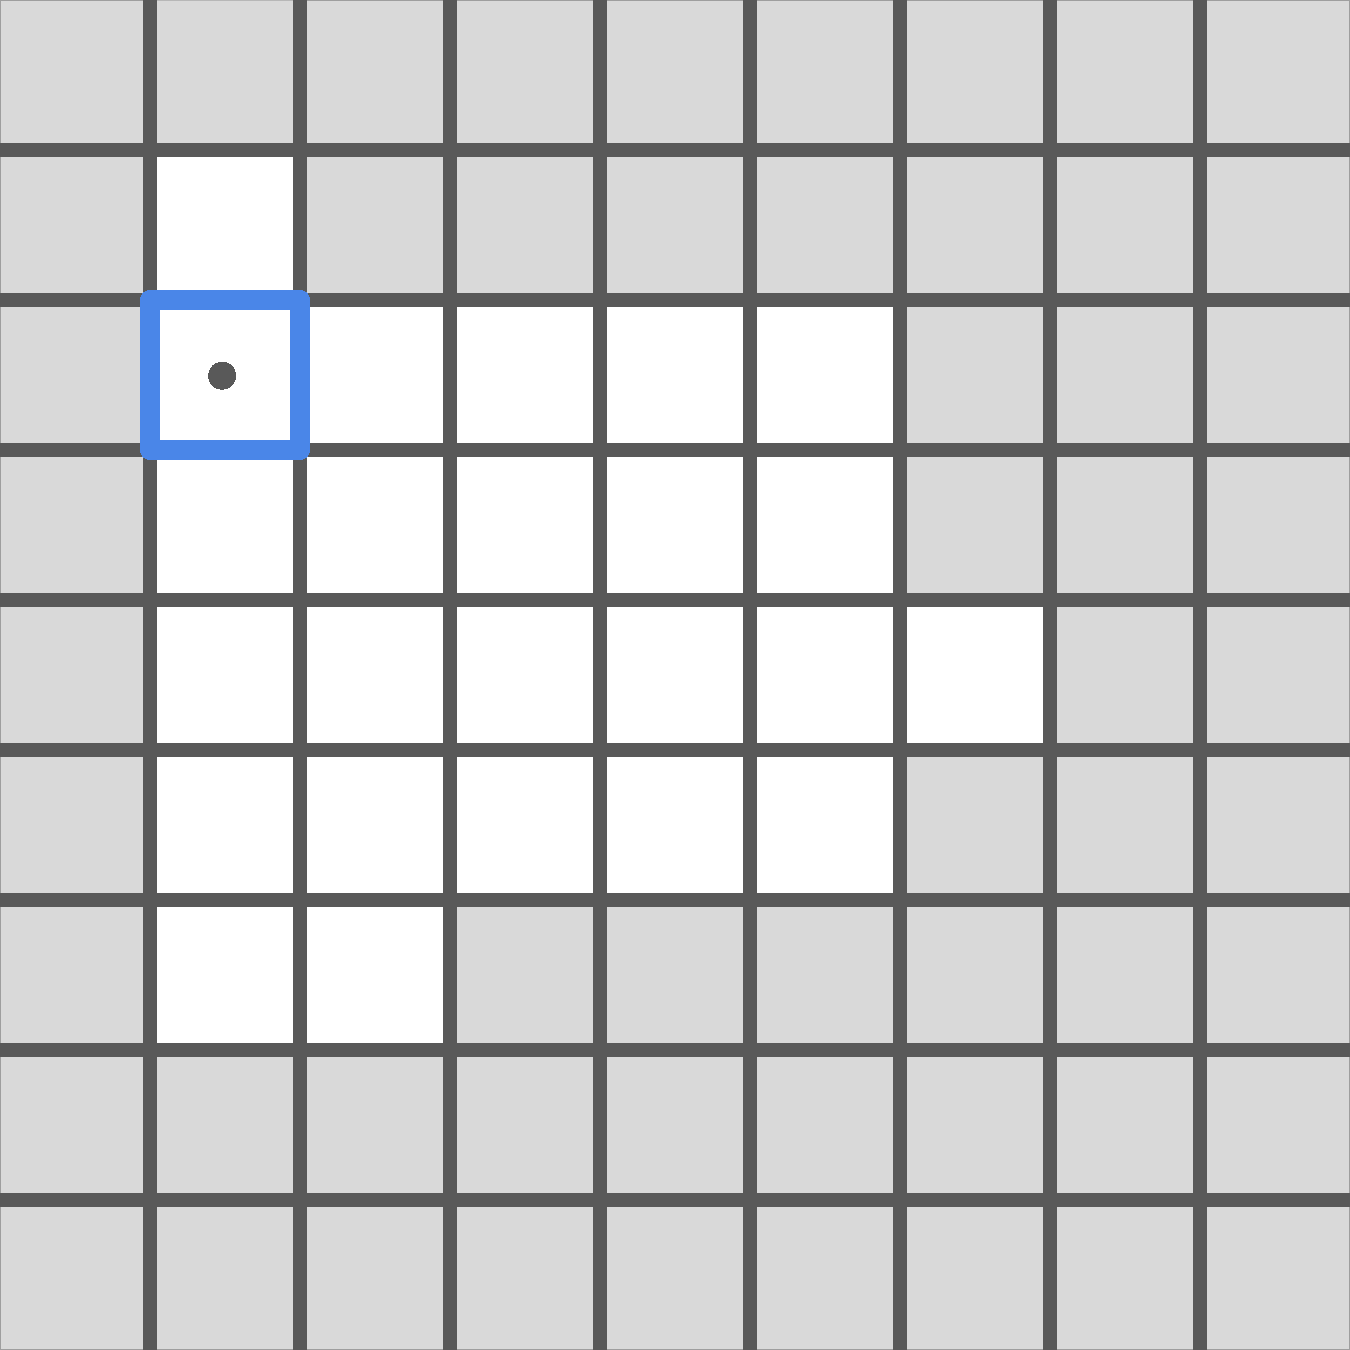
\includegraphics[width=\linewidth,trim={0 100 100 0},clip]{spiker-diagram/spiker-generate}
  \caption{cell buds developmental search prongs}
  \label{fig:spiker-generate}
\end{subfigure}
	\hspace{2ex}
\begin{subfigure}[t]{0.25\linewidth}
  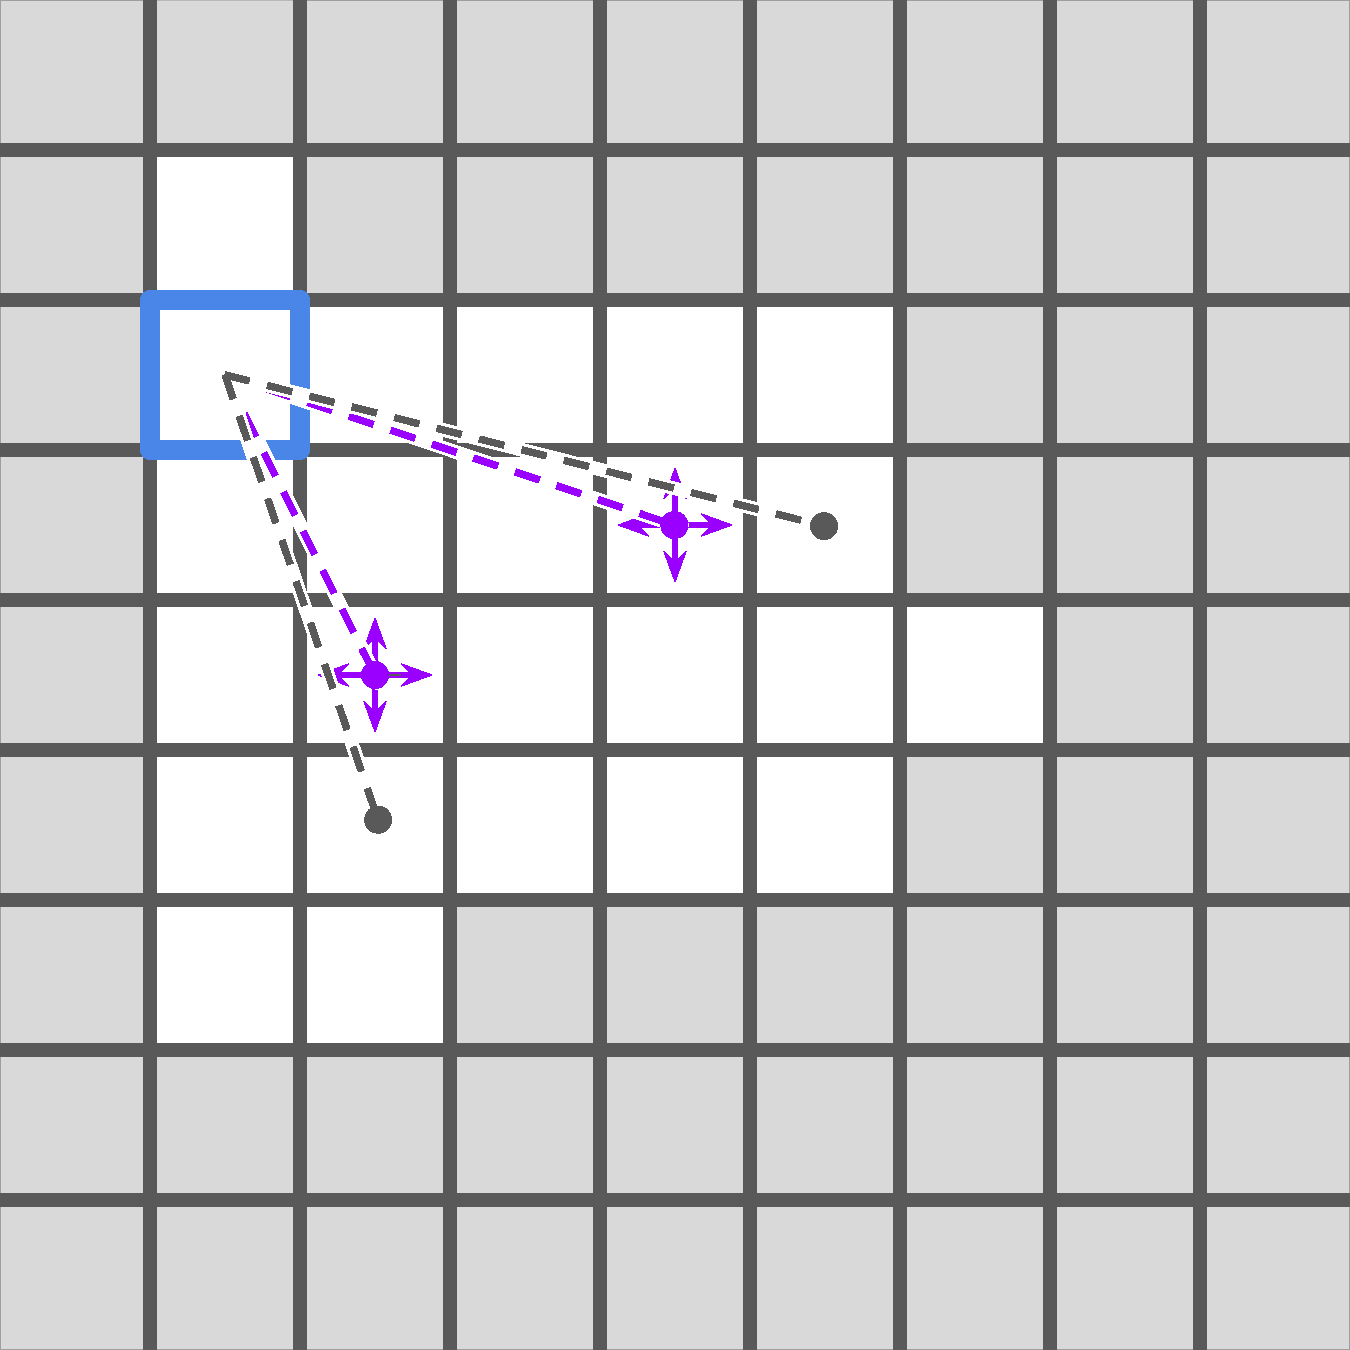
\includegraphics[width=\linewidth,trim={0 100 100 0},clip]{spiker-diagram/spiker-walk}
  \caption{search prongs perform random walk}
  \label{fig:spiker-walk}
\end{subfigure}
  \hspace{2ex}
\begin{subfigure}[t]{0.25\linewidth}
  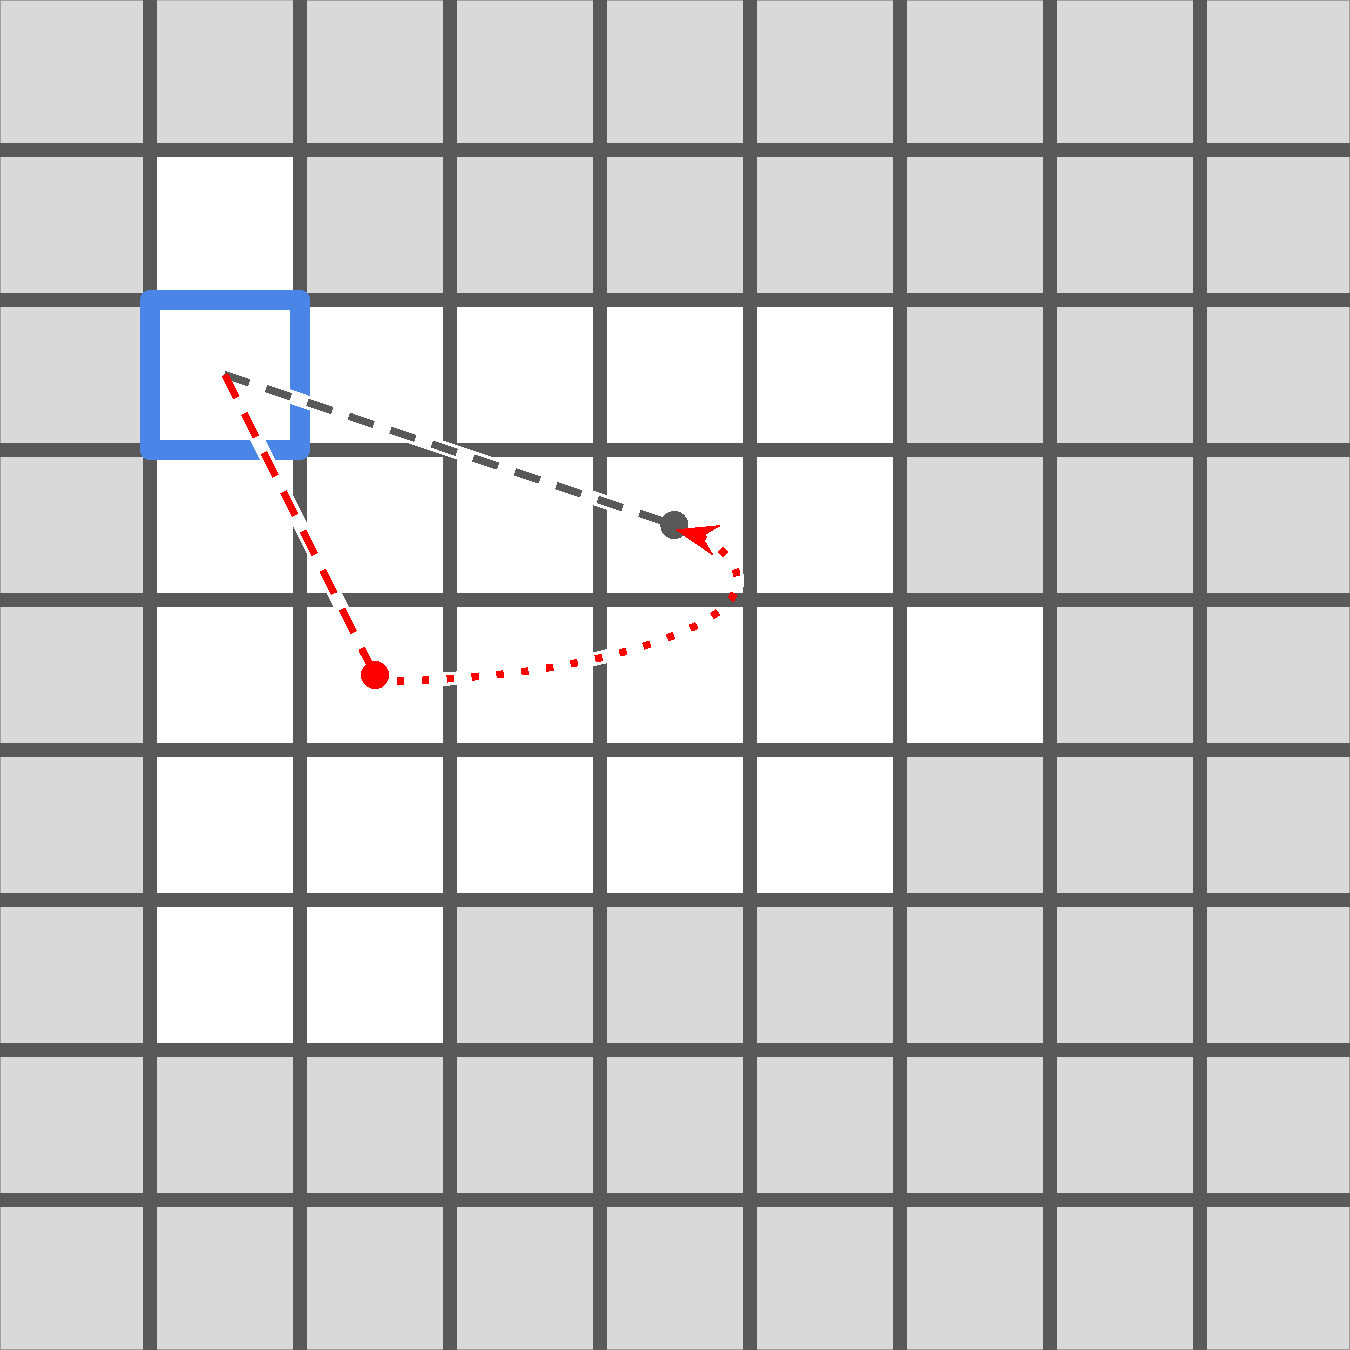
\includegraphics[width=\linewidth,trim={0 100 100 0},clip]{spiker-diagram/spiker-swap}
  \caption{poorly-performing prong resets to better-performing prong}
  \label{fig:spiker-swap}
\end{subfigure}
\end{center}
\end{minipage}

\begin{minipage}{\linewidth}
\begin{center}
\begin{subfigure}[t]{0.25\linewidth}
  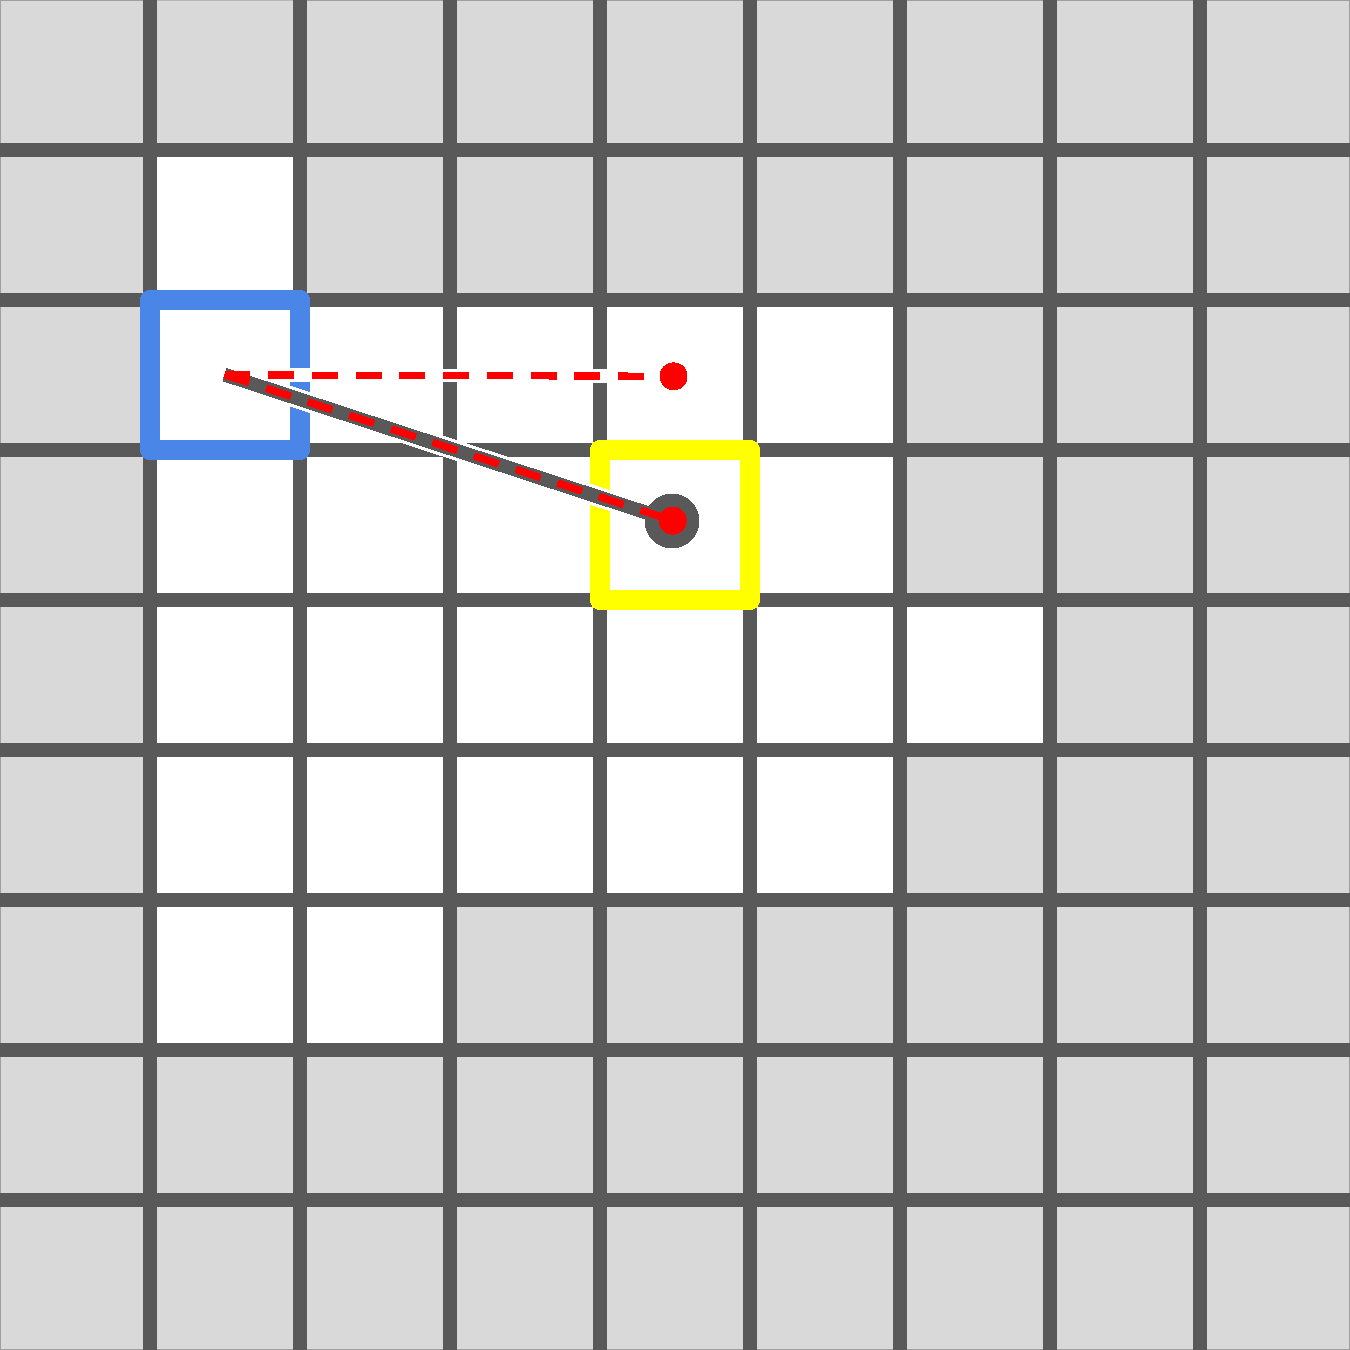
\includegraphics[width=\linewidth,trim={0 100 100 0},clip]{spiker-diagram/spiker-connect}
  \caption{search prong matures into established connection}
  \label{fig:spiker-connect}
\end{subfigure}
  \hspace{2ex}
\begin{subfigure}[t]{0.25\linewidth}
  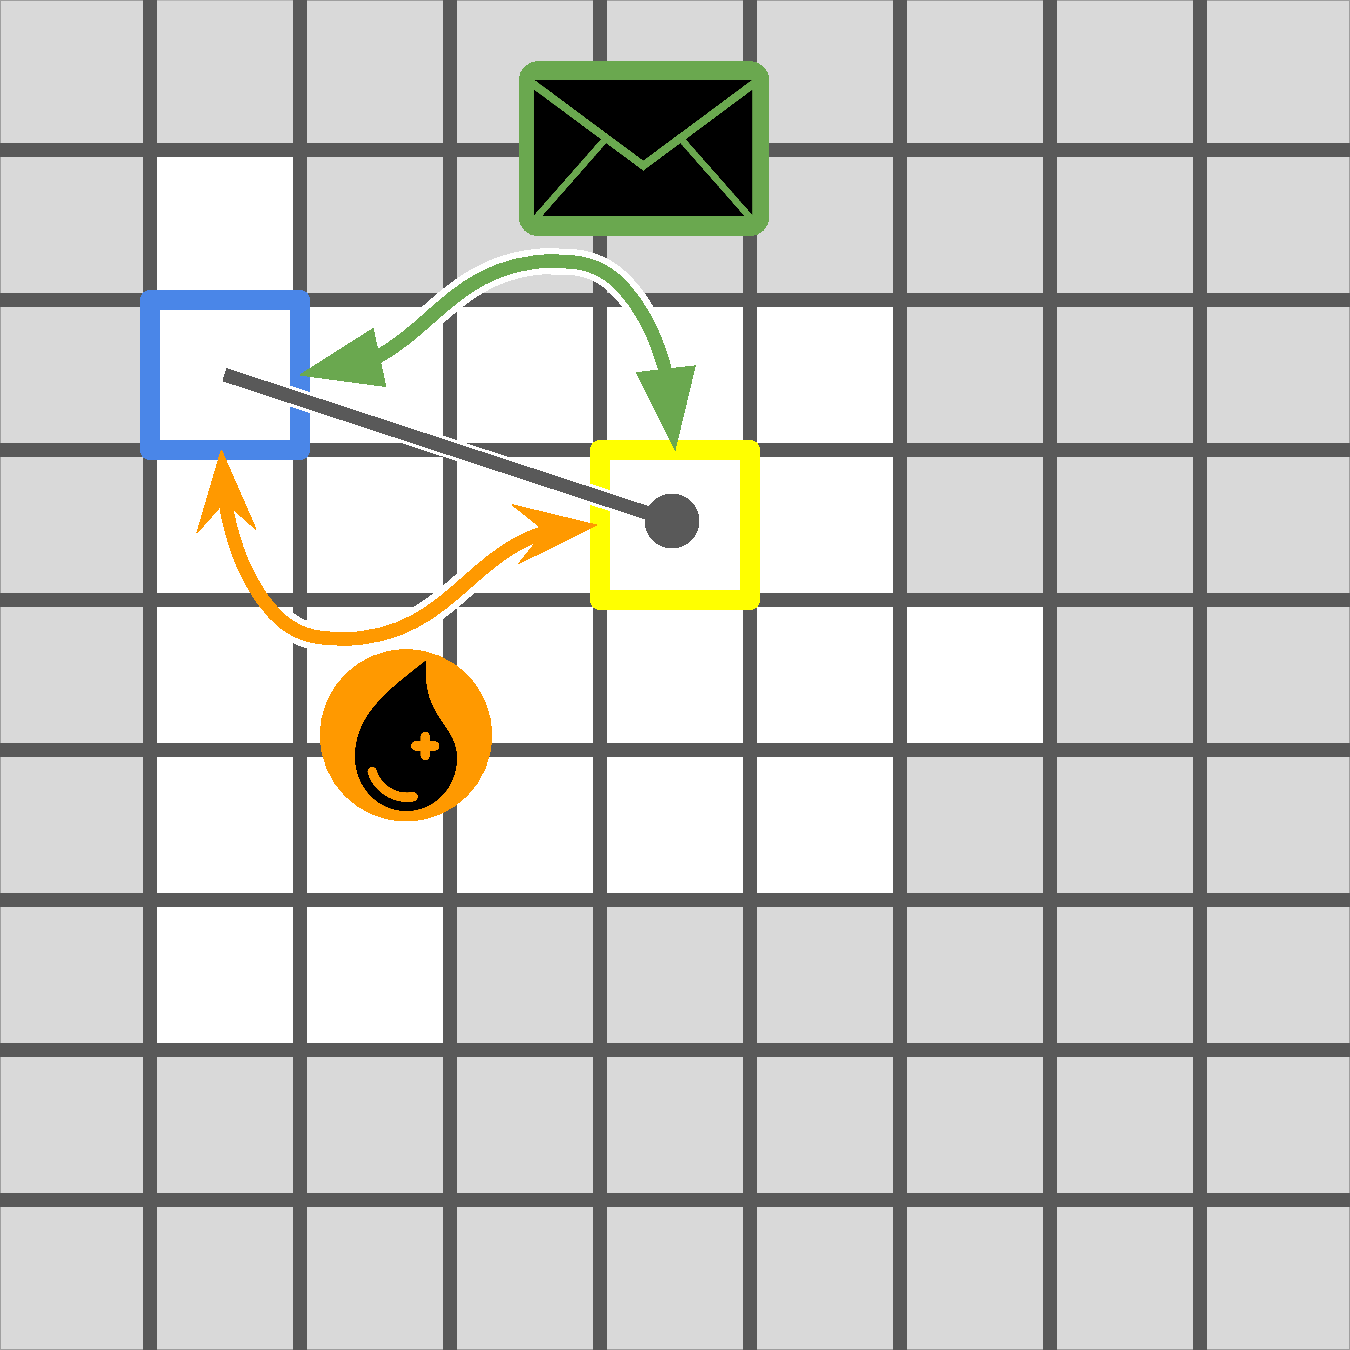
\includegraphics[width=\linewidth,trim={0 100 100 0},clip]{spiker-diagram/spiker-transmit}
  \caption{cells exchange messages over established interconnect}
  \label{fig:spiker-transmit}
\end{subfigure}
   \hspace{2ex}
\begin{subfigure}[t]{0.25\linewidth}
  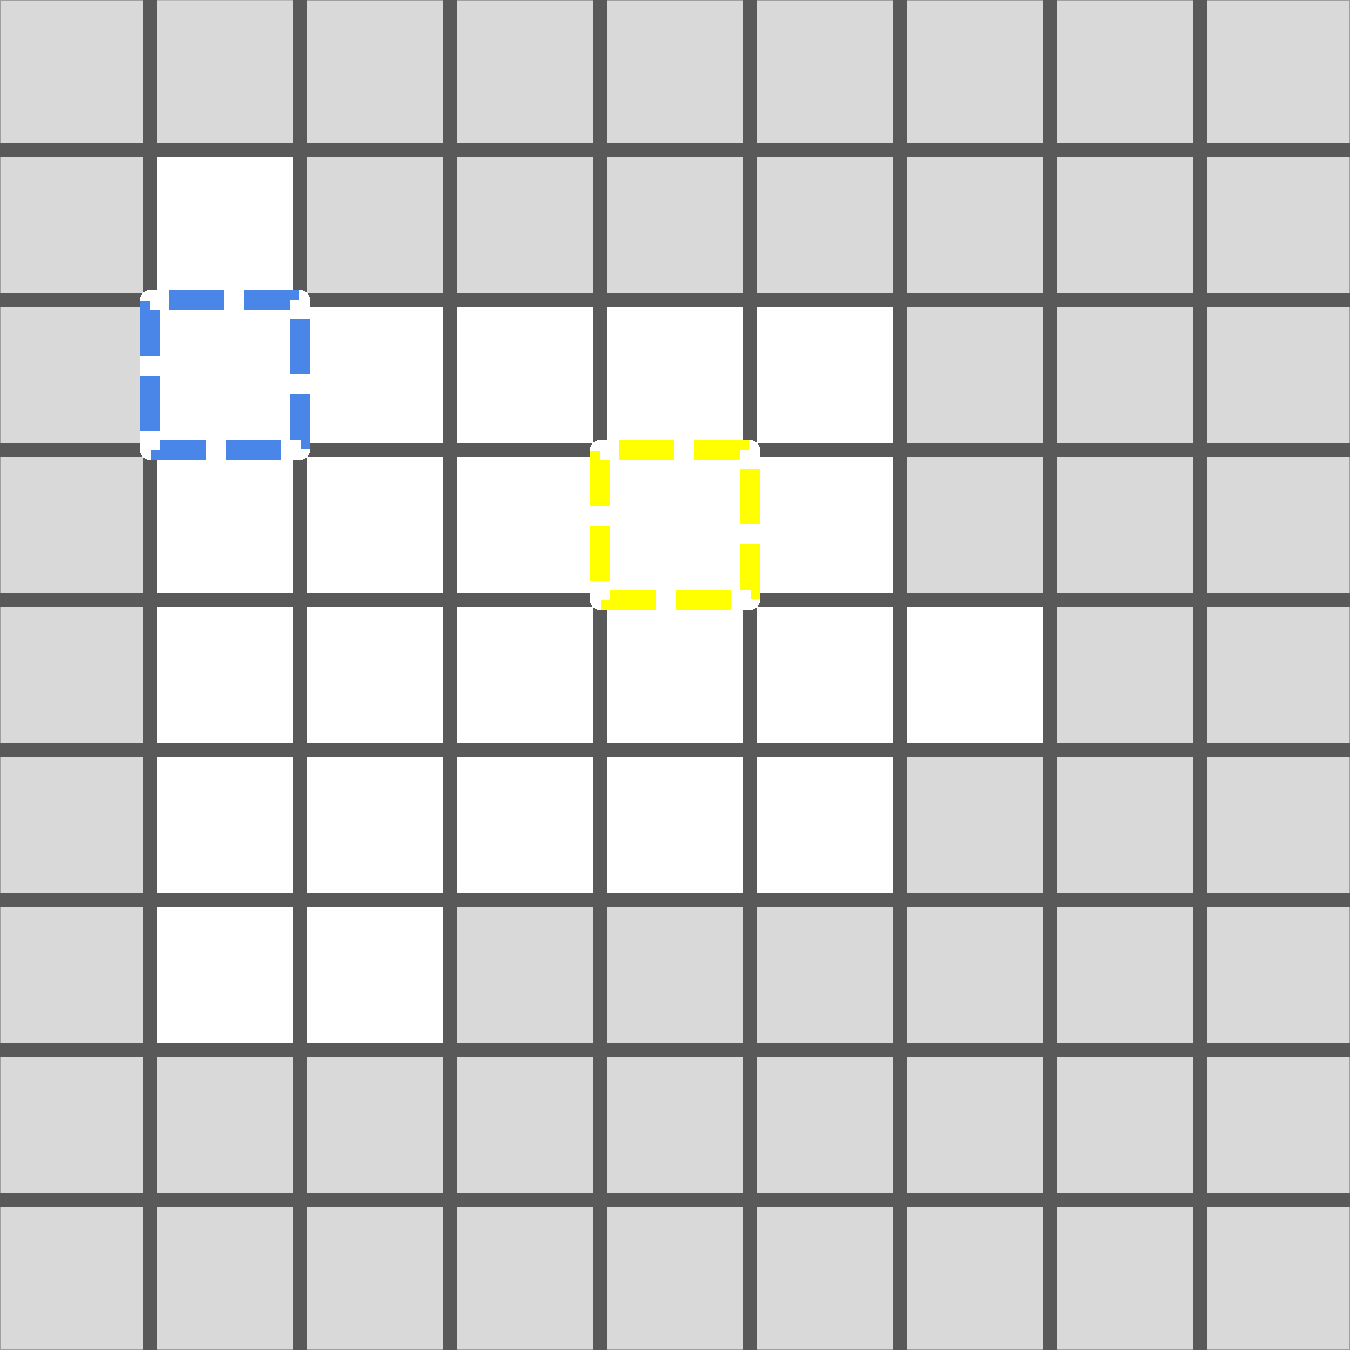
\includegraphics[width=\linewidth,trim={0 100 100 0},clip]{spiker-diagram/spiker-remove}
  \caption{established interconnects may be removed by either participating cell}
  \label{fig:spiker-remove}
\end{subfigure}
\end{center}
\end{minipage}

\caption{
Illustration of the developmental process used to establish long-distance interconnects.
You can see this developmental process in action in an evolved strain at \url{https://mmore500.com/hopto/ap}.
}
\label{fig:spiker_diagram}
\end{center}
\end{figure}

\fi




%%% HERE IS THE REAL FIGURE!
%\iffalse

\begin{figure}[!htbp]
\begin{center}
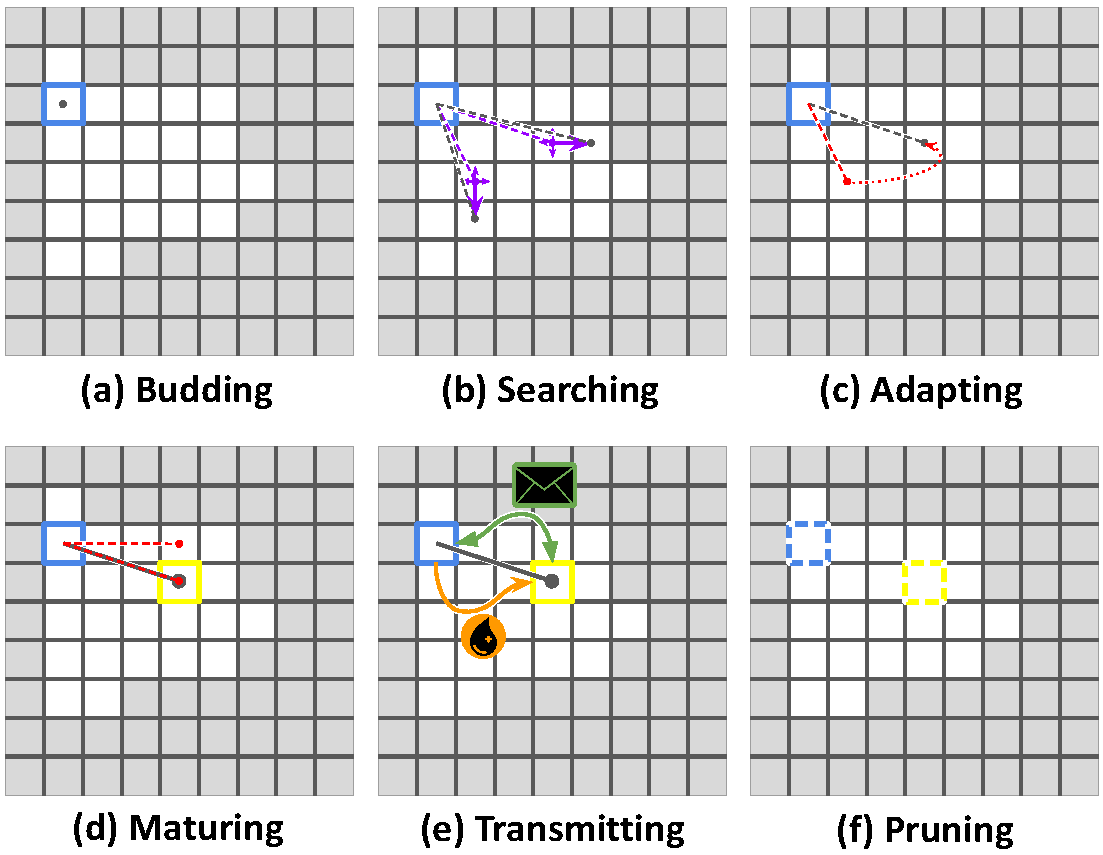
\includegraphics[width=1.0\linewidth]{img/spiker-diagram/spiker-combined.pdf}
\caption{
Illustration of the developmental process used to establish long-distance interconnects.  Cells start by budding developmental search prongs (a) that perform a random search (b), reverting to the most successful search (c) where it matures to establish a connection (d).  Messages and resources can be transmitted over a connection (e) until either cell decides to terminate the connection (f).
You can see this developmental process in action in an evolved strain at \url{https://mmore500.com/hopto/ap}.
}
\label{fig:spiker_diagram}
\end{center}
\end{figure}

%\fi
